Now that we've seen the main physical part of our Rocket as the PCB and the
physics in the appendix. Let's go back to our specifications. Our rocket needs
to support up to 16g of acceleration, we need to acquire the flight data and
finally we need our rocket to be stabilized by 4 ailerons. We'll now talk about
this last part. For a more efficient read about this I'll present you with the
plan that we will follow:

\begin{itemize}
    \item The control theory behind controlling said ailerons and how to integrate those
          equations into simulation software
    \item The application and translation of those simulations to the software.
\end{itemize}

After those three axes we will finally conclude about the controller side of
the rocket.

To finish this introduction, you will see below a schematic of Opale. The
ailerons that we will control are the forwardmost ones. There are not many
reasons apart from the challenge to use such ailerons at the front of a micro
test rocket as the inherent stability of a rocket would be enough for most
rockets of this size. Those ailerons even reduce this stability by firstly
reducing the ratio CG/CP (center of gravity per center of portance, see the
mechanical appendix for more detail). The reason to add such ailerons for our
project is to first and foremost add the challenge and complexity needed for
this project to be worthy of being a TER and secondly in the future, we could
change the software to follow some sort of waypoints in the air for the rocket
to try and follow.

\begin{figure}[!hbt]
    \centering
    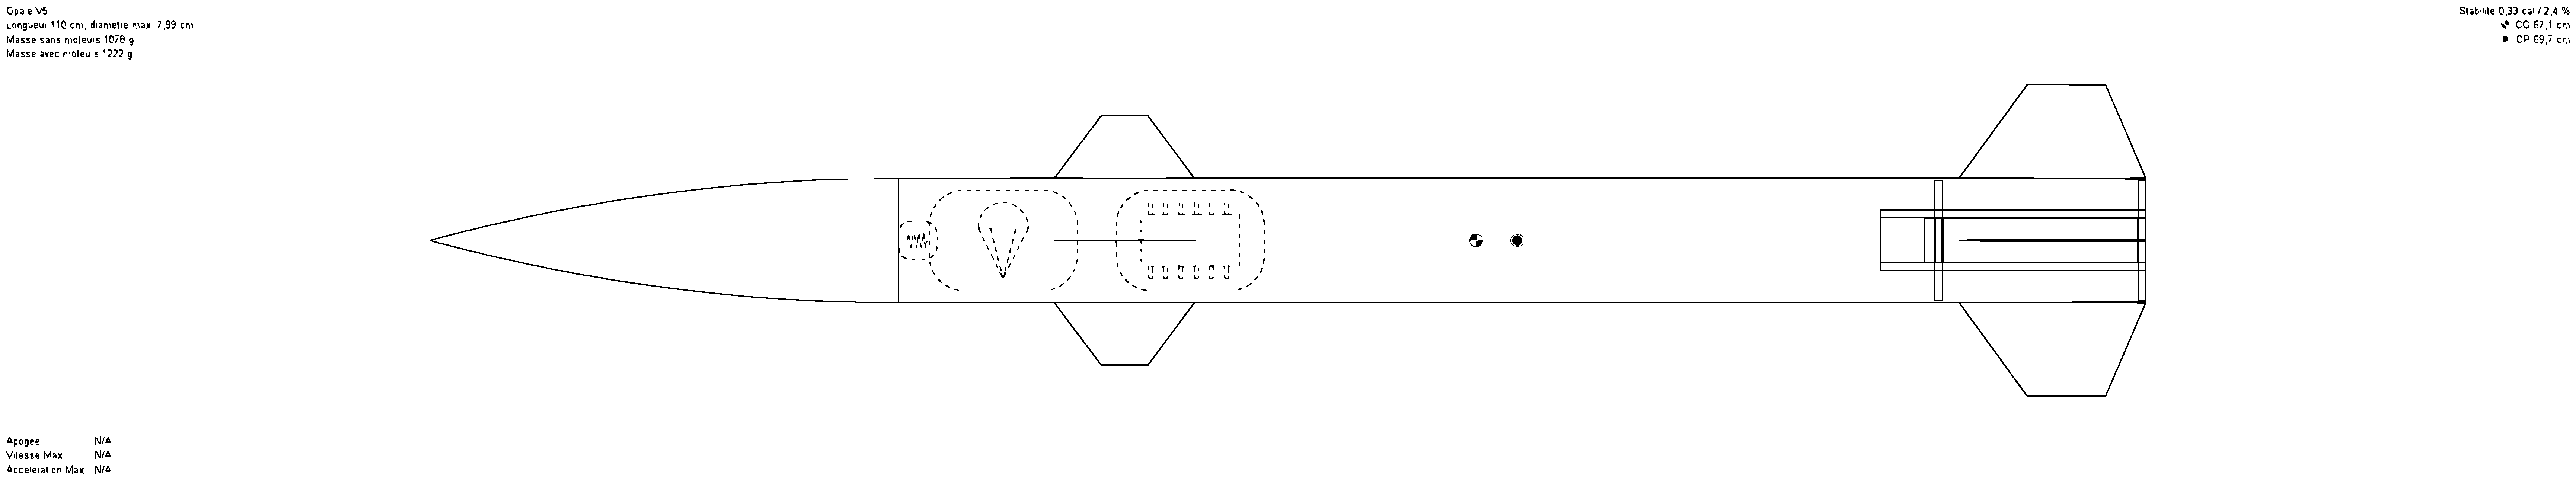
\includegraphics[width=\SchematicWidth]{\Images/mechanical/RocketSchematics.eps}
    \caption{Mechanical schematic of the rocket}
\end{figure}
\FloatBarrier

% Control theory input
\section{The control theory and integration into simulation}
We will now talk about the equations and the control theory behind Opale to be
able to simulate it later and to better comprehend what physical phenomenon
will impact the flight of our rocket to be more precise in the conception of
the body. One thing to be noted is that we will use Euler's equation to
comprehend those

\subsection{Simplified Dynamics of the Rocket with 3 DoF}

\begin{figure}
    \centering
    \resizebox{\SchematicWidth}{!}{%
        \begin{tikzpicture}
            % adding grid
            \draw [->, line width=0.5pt] (0,-0.5) -- (0,10) node [left] {Z};
            \draw [->, line width=0.5pt] (-0.5,0) -- (10,0) node [below] {X};

            % Adding arrows
            % Horizontals
            \draw[->, line width=2pt] (5.8,0) -- (4,0) node[midway, below]{\(-R\cos{\theta}\)};
            \draw[->, line width=2pt] (6.2,0) -- (8,0) node[midway,below] {\(Pcos{\theta}\)};
            % Vertical
            \draw[->, line width=2pt] (0,5.8) -- (0,4) node[left] {\(-R\sin{\theta}\)};
            \draw[->, line width=2pt] (0,5.8) -- (0,4.4) node[left] {\(-M_g\)};
            \draw[->, line width=2pt] (0,6.2) -- (0,8) node[left] {\(P\sin{\theta}\)};

            % small lines that make the graphe readable
            % Horizontal lines
            \draw [dotted, line width=0.5pt] (0.5,4) -- (4,4);
            \draw [dotted, line width=0.5pt] (0.5,6) -- (6,6);
            \draw [dotted, line width=0.5pt] (0.5,4.4) -- (6, 4.4);
            \draw [dotted, line width=0.5pt] (0.5,8) -- (8,8);
            % Vertical lines
            \draw [dotted, line width=0.5pt] (4,0.5) -- (4,4);
            \draw [dotted, line width=0.5pt] (5.6,0.5) -- (5.6,5.6);
            \draw [dotted, line width=0.5pt] (6,0.5) -- (6,6);
            \draw [dotted, line width=0.5pt] (8,0.5) -- (8,8);

            % Adding the rocket
            \path [draw=black, fill=yellow, line width=0.1mm]
            (4.625,3.875) -- ++(0.6,0.6) -- ++(0,0.5) -- ++(1.1,1.1) --
            ++ (0.5,0.75) -- ++(-0.75,-0.5) -- ++(-1.1,-1.1) --
            ++ (-0.5,0) -- ++(-0.6,-0.6) -- ++(0.5,0) -- ++(0.25,-0.25)
            -- ++(0,-0.5);

            % Adding forces vector
            \draw [->, line width=1pt] (5.6,5.6) node [above left] {CP}-- (4,4) node [below left] {\(\overrightarrow{R}\)};
            \draw [->, line width=1pt] (6,6) -- (8,8) node [above] {\(\overrightarrow{P}\)};
            \draw [->, line width=1pt] (6,6) node [below right] {CG} -- (6,4.4) node [right] {\(\overrightarrow{M_g}\)};

            % Adding angle mark
            \draw (1,1) coordinate(B) -- (2,1) coordinate(A);
            \draw (1,1) -- (2,2) coordinate(C);
            \pic [draw, ->, "$\theta$", angle eccentricity=1.5] {angle = A--B--C};

        \end{tikzpicture}
    }
    \caption{Forces applied to the rocket}\label{img:rocket_forces}
\end{figure}

\FloatBarrier

This rocket can be modeled as a rigid body with 3 degrees of freedom (DoF), but
the control can be focused primarily on pitch and yaw. To follow everything
below we will now see about a 3D case of our rocket this part has been heavily
inspired by the document “Le vol de la Fusée, Stabilité et Trajectographie” by
the CNES \ref{img:rocket_forces}.

If we look a bit into the forces on the rocket in flight we can get the figure
just above and we can take out those 2D equations rather easily:

\begin{minipage}[c]{1\textwidth}
    \centering
    \begin{align*}
        P_x      & = P \times \cos({\theta})   \\
        R_x      & = - R \times \cos({\theta}) \\
        P_z      & = P \times \sin({\theta})   \\
        Weight_Z & = -M \times g               \\
        R_z      & = -R \times \sin ({theta})  \\
    \end{align*}
\end{minipage}
\FloatBarrier

Now that we have our basic equations, we can determine our equations based on
time and in 3D :

\begin{minipage}[c]{1\textwidth}
    \centering
    \begin{align*}
        t_i  & = t_{i-1} + dt \text{: Compute the actual time}                                                                      \\
        m_i  & = m_{i-1} - dm \text{: compute the mass of the roceket as the motor burns fuel}                                      \\
        P_i  & = \text{mean thrust between $t_i$ and $t_{i-1}$}                                                                     \\
        Fr_i & = (P_i - \frac{1}{2}\rho(Z_{i-1}SCx(V_{i-1})V^2_{i-1}) \cos({\text{pitch}_{i-1}})) \text{: Horizontal sum of forces} \\
        Fz_i & = (P_i - \frac{1}{2}\rho(Z_{i-1}SCx(V_{i-1})V^2_{i-1}) \sin({\text{pitch}_{i-1}})) \text{: Vertical sum of forces}   \\
        Gr_i & = \frac{Fr_i}{m_i} \text{: Horizontal acceleration}                                                                  \\
        Gz_i & = \frac{Fz_i}{m_i} \text{: Vertical acceleration}                                                                    \\
        Vr_i & = Vr_{i-1} + Gr_i dt \text{: Horizontal velocity}                                                                    \\
        Vz_i & = Vz_{i-1} + Gz_i dt \text{: Vertical velocity}                                                                      \\
        V_i  & = \sqrt{Vr_i^2 + Vz_i^2} \text{: Total velocity}                                                                     \\
        X_i  & = X_{i-1} + (Vr_i dt + Gr_i \frac{dt^2}{2}) \cos({yaw})\text{: X position}                                           \\
        Y_i  & = Y_{i-1} + (Vr_i dt + Gr_i \frac{dt^2}{2}) \sin({yaw}) \text{: Y position}                                          \\
        Z_i  & = Z_{i-1} + Vzi dt + Gz_i \frac{dt^2}{2} \text{: Z position}                                                         \\
    \end{align*}
\end{minipage}

And, for the pitch :
\begin{itemize}
    \item If the rocket left the launch ramp :
          \begin{itemize}
              \item \begin{gather*}
                        pitch_i  = \arctan{V_{z_i}}{V_{r_i}}
                    \end{gather*}
          \end{itemize}
    \item If the rocket is on the launch ramp
          \begin{itemize}
              \item \begin{align*}
                        Fr_i & = Fr_i - m_i \times g \times cos({pitch_{i-1}}) \times sin({pitch_{i-1}}) \\
                        Fz_i & = Fz_i - m_i \times g \times cos({pitch_{i-1}}) \times cos({pitch_{i-1}}) \\
                    \end{align*}
          \end{itemize}
\end{itemize}

\newpage % Get new page for the flowchart
Those equations can be exported into simulation software like Simulink
following this flow chart :

\begin{figure}[!ht]
    \centering
    \resizebox{0.75\textwidth}{!}{%
        \begin{circuitikz}
            \tikzstyle{every node}=[font=\large]
            \draw [ fill={rgb,255:red,168; green,255; blue,168} ] (12.5,30.75) rectangle  node {\large $\text{Start of calculations :} M_0, V_0, Z_0, \theta_0$} (25,28.25);
            \draw [ fill={rgb,255:red,125; green,190; blue,255} ] (12.5,25.75) rectangle  node {\large $\text{Calculate} M_i$} (25,23.25);
            \draw [ fill={rgb,255:red,125; green,190; blue,255} ] (5,20.75) rectangle  node {\large $\text{Calculate} \gamma X_i (\text{Depends} n R_{i-1} and cos \theta_{i-1})$} (17.5,18.25);
            \draw [ fill={rgb,255:red,125; green,190; blue,255} ] (20,20.75) rectangle  node {\large $\text{Calculate} \gamma Y_i (\text{Depends} n R_{i-1} and sin \theta_{i-1})$} (32.5,18.25);
            \draw [ fill={rgb,255:red,125; green,190; blue,255} ] (5,15.75) rectangle  node {\large $\text{Calculate} V\gamma_i (\text{Depends on} Vx and \gamma_i)$} (17.5,13.25);
            \draw [ fill={rgb,255:red,125; green,190; blue,255} ] (20,15.75) rectangle  node {\large $\text{Calculate} Vz_i (\text{Depends on} Vz_{i-1} and \gamma_i )$} (32.5,13.25);
            \draw [ fill={rgb,255:red,125; green,190; blue,255} ] (5,10.75) rectangle  node {\large $\text{Calculate} the x_i (\text{Depends on} X_{i-1} and \gamma X_i)$} (17.5,8.25);
            \draw [ fill={rgb,255:red,125; green,190; blue,255} ] (20,10.75) rectangle  node {\large $\text{Calculate} Z_i (\text{Depends on} Z_{i-1} and \gamma Z_i)$} (32.5,8.25);
            \draw [ fill={rgb,255:red,125; green,190; blue,255} ] (12.5,5.75) rectangle  node {\large $\text{Calculate} V_i$} (25,3.25);
            \draw [ fill={rgb,255:red,125; green,190; blue,255} ] (12.5,0.75) rectangle  node {\large $\text{Calculate} R_i$} (25,-1.75);
            \draw [ fill={rgb,255:red,125; green,190; blue,255} ] (12.5,-4.25) rectangle  node {\large $\text{Calculate} \theta_i$} (25,-6.75);
            \draw [ fill={rgb,255:red,251; green,223; blue,249} ] (12.5,-9.25) rectangle  node {\large Does the rocket has landed ?} (25,-11.75);
            \draw [ fill={rgb,255:red,255; green,128; blue,128} ] (12.5,-14.25) rectangle  node {\large End of calculations} (25,-16.75);
            \draw [->, >=Stealth] (18.75,28.25) -- (18.75,25.75);
            \draw [->, >=Stealth] (11.25,22) -- (11.25,20.75);
            \draw [->, >=Stealth] (26.25,22) -- (26.25,20.75);
            \draw [->, >=Stealth] (11.25,18.25) -- (11.25,15.75);
            \draw [->, >=Stealth] (26.25,18.25) -- (26.25,15.75);
            \draw [->, >=Stealth] (11.25,13.25) -- (11.25,10.75);
            \draw [->, >=Stealth] (26.25,13.25) -- (26.25,10.75);
            \draw [->, >=Stealth] (18.75,7) -- (18.75,5.75);
            \draw [->, >=Stealth] (18.75,3.25) -- (18.75,0.75);
            \draw [->, >=Stealth] (18.75,-1.75) -- (18.75,-4.25);
            \draw [short] (11.25,22) -- (26.25,22);
            \draw [short] (18.75,23.25) -- (18.75,22);
            \draw [short] (11.25,8.25) -- (11.25,7);
            \draw [short] (11.25,7) -- (26.25,7);
            \draw [short] (26.25,8.25) -- (26.25,7);
            \draw [->, >=Stealth] (18.75,-6.75) -- (18.75,-9.25);
            \draw [->, >=Stealth] (18.75,-11.75) -- (18.75,-14.25)node[pos=0.5, fill=white]{YES};
            \draw [short] (12.5,-10.5) -- (2.5,-10.5)node[pos=0.5, fill=white]{NO};
            \draw [short] (2.5,-10.5) -- (2.5,24.5);
            \draw [->, >=Stealth] (2.5,24.5) -- (12.5,24.5);
        \end{circuitikz}
    }%
    \caption{Algorithm used to simulate the rocket trajectory.}
    \label{fig:my_label}
\end{figure}
\subsection{The rotational equation to make our model with 6DoF}

We now have our equations to compute the position and its derivatives over
time. The thing is those equations are only for a rigid body with only 3 DoF
and without any ailerons added to them. To be able to have our 6 DoF and to be
able to input our ailerons into this simulation we need to refer to Euler's
equation of rotational dynamics as well as the standard aerodynamic lift
equations:

For a rigid body\footnote{rigid body is symmetrical and the axes are aligned
    with the frame} with a diagonal inertia tensor:
\begin{gather*}
    \begin{cases}
        r_x = I_x \dot{\omega}_x - (I_y - I_z)\omega_y \omega_z \\
        r_y = I_y \dot{\omega}_y - (I_z - I_x)\omega_z \omega_x \\
        r_z = I_z \dot{\omega}_z - (I_x - I_y)\omega_x \omega_y
    \end{cases}
\end{gather*}

with $r$ the net torque, $I_\omega$ the angulor momentum, $I$ the inertia
tensor and $\omega$ is the angular velocity.

We can assume that the rocket is symmetrical so $I_x=I_y$ and we could
calculate the $I_z$ but we would see that if the rocket is long but slim it
tends to be small. We consider as well that the pitch and yaw are coupled but
the roll isn't coupled with the rest.

We now find thoses equations :
\begin{gather*}
    \begin{cases}
        r_x = I_x \dot{\omega}_x - (I_x - I_z)\omega_y \omega_z \\
        r_y = I_x \dot{\omega}_y - (I_z - I_x)\omega_z \omega_x \\
        r_z = I_z \dot{\omega}_z
    \end{cases}
\end{gather*}

We can integrate those equations into the simulation like this:

\begin{align*}
    \dot{\omega}_x & = \frac{1}{I_x}(r_x + (I_x - I_z)\omega_y \omega_z) \\
    \dot{\omega}_y & = \frac{1}{I_x}(r_y + (I_z - I_x)\omega_z \omega_x) \\
    \dot{\omega}_z & = \frac{I_z}r_z                                     \\
\end{align*}

And we can integrate them over time to get orientation rates like this :

\begin{gather*}
    \dot{\omega}_i(t + dt) = \omega_i(t) + \dot{\omega}_i dt
\end{gather*}

Because we use Euler's equations, we encounter a problem known as the gimbal
lock. This happens as two rotation axes become aligned. Because we are in a 3D
space instead of a 4D space like for quaternions, we can't differentiate
between those two axes and so we lose a DoF as long as those axes are merged.

% Aerodynamics
\subsection{Aerodynamics equations for the ailerons}

Now for the ailerons we choosed the NACA-0009 at 9\% fill design for ailerons,
which is used for most control surfaces of this size because it grants a
sufficient lift coefficient as well as a good linear lift region. It grants
about 14 to 16 degrees before our aileron stalls. We assume that this is with a
relatively high number of Reynolds which we have a chord of 9 cm. We can see
this thanks to this equation :

\begin{gather*}
    R_e = \frac{\rho V c}{\mu}
\end{gather*}

with $c$ the chord lenght and $V$ the airflow on the ailerons.

So, with our rocket going at max at $130 \si{\meter\per\second}$ and with a
chord length of $9 \si{\centi\meter}$ we have $8.05 \times 10^{-5} Re$ which is
considered high ($10^5 \text{ to } 10^6 \space Re$ is considered high in
aviation) we can also calculate that our ailerons would have a flow separation
between each side of the ailerons at approximately $10 \si{\degree}$ to $12
    \si{\degree}$ of angle of attack (AoA) which would render our control of the
flow non-linear. So, with this in mind we can limit our AoA at 10° at most in
the embedded code as well as in the simulation.

\begin{figure}[!hbt]
    \centering
    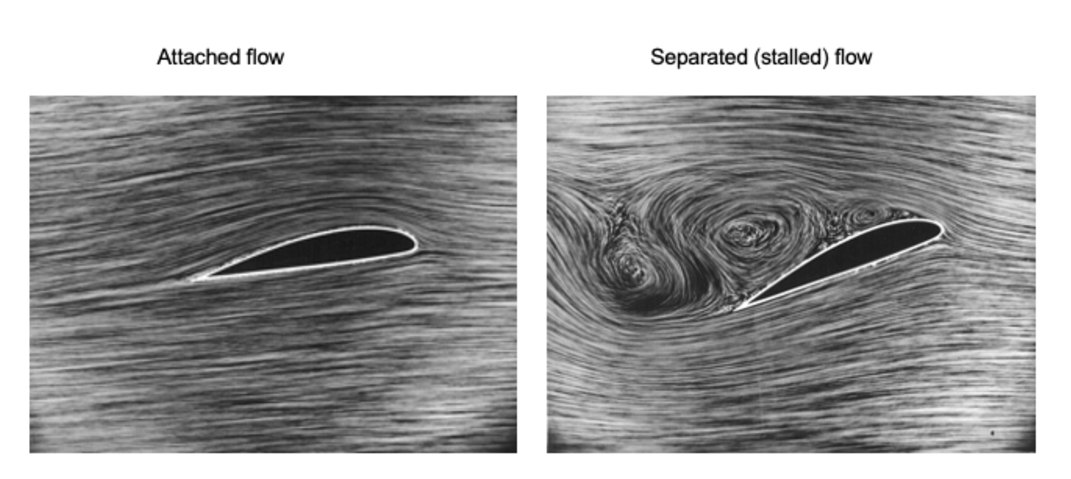
\includegraphics[width=\SchematicWidth]{\Images/mechanical/AirfloilStall.eps}
    \caption{Mechanical schematic of the rocket}
\end{figure}
\FloatBarrier

Now to be able to simulate those ailerons we need to be able to calculate the
torque generated by each aileron to add into the equation of rotation we saw
just above. For each aileron we can determine their impact on the total torque
generated with :

\begin{align*}
    F_L  & = \frac{1}{2} \rho V^2 S C_L (\delta)                     \\
    \tau & = r * F_L                                                 \\
         & = r ( \frac{1}{2} \rho V^2 S C_{L \delta} \times \delta)  \\
         & = \frac{1.006 \times 160 \times 0.09}{1.8 \times 10^{-5}} \\
         & = 8.05 \times 10^{-5}                                     \\
\end{align*}

We can say that :

\begin{gather*}
    K_\tau = \frac{1}{2} \rho V^2 S C_{L \delta} r
\end{gather*}

And thus:

\begin{gather*}
    \tau = K_\tau \times \delta
\end{gather*}

With $V$ the velocity, $S$ the surface $C_{L \delta}$ the derivative of the
lift coefficient, $F_L$ the lift force, $\tau$ the torque, $K_\tau$ the control
effectiveness coefficient, $\delta$ the AoA and r the moment arm which is the
distance between the $CL$ and the $CM$ of the rocket.

To integrate those equations into the simulation we only must determine the
angles of our ailerons over time and input it in the previous equations :

\begin{gather*}
    \tau_i = \frac{1}{2} \rho V^2 S C_{L \delta} r \times \delta_i
\end{gather*}

Our $\delta_i$ will be computed through the output of our simulated PID which
we will see just below this.

With this we can now create our own simulation. We just need to add a few
gaussian noise generators to our system to test our resistance to noise, a
thrust curve to input our thruster in there and a delay between the controller
and the actuators to test even further our model. Which can resemble this:

\begin{figure}[!hbt]
    \centering
    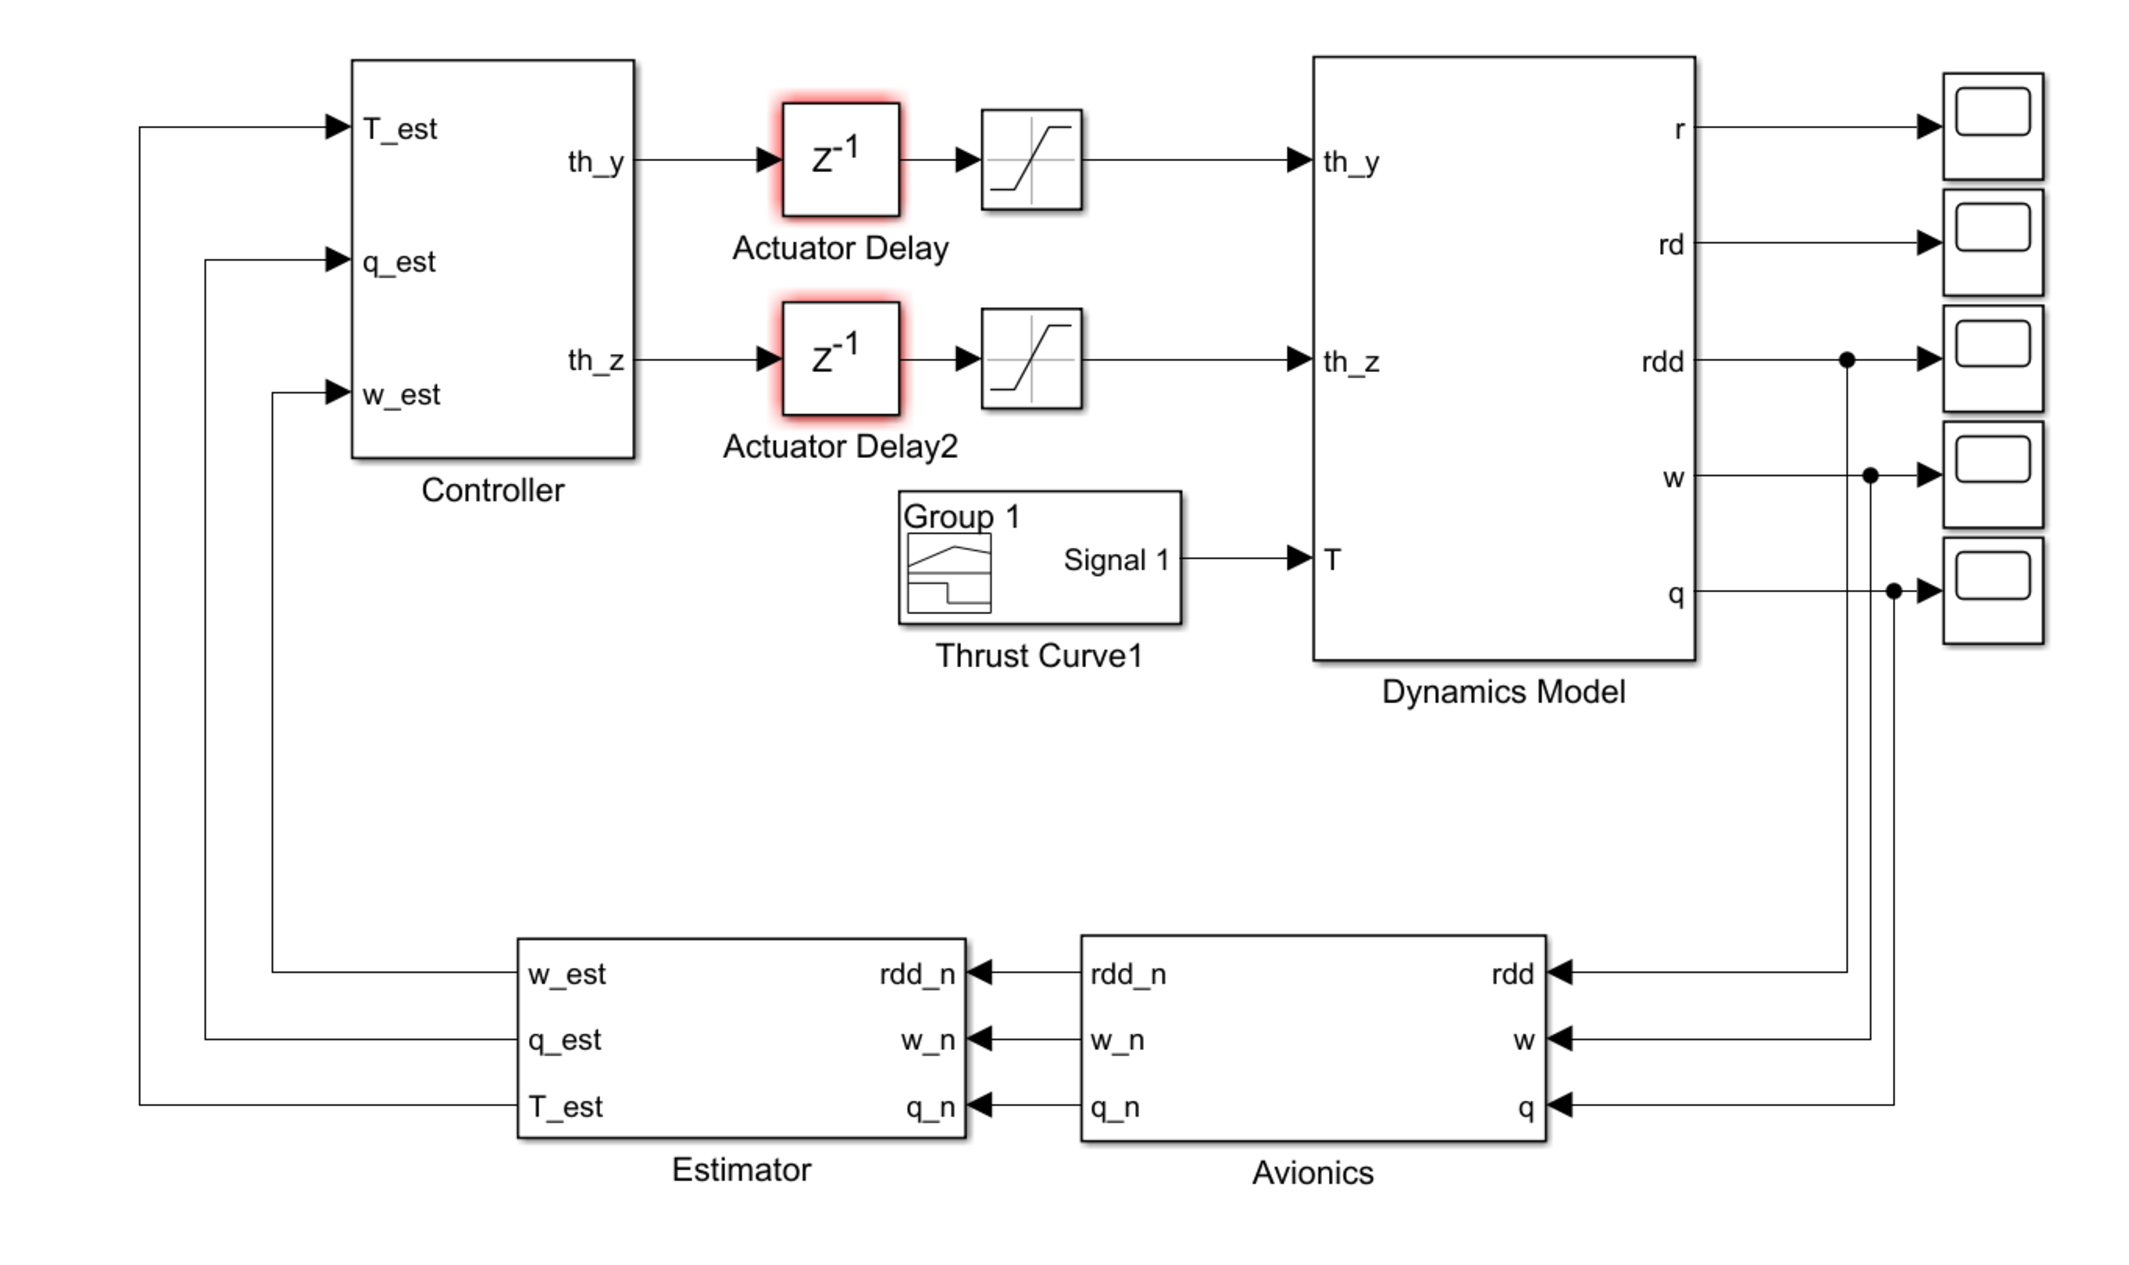
\includegraphics[width=\SchematicWidth]{\Images/rocket_sim/simulink.eps}
    \caption{Simulink model we used}
\end{figure}
\FloatBarrier

To complete our simulation and to be able to compute the angles of every
aileron we need to have some sort of controller. In our case, we will use a PID
controller as it is the controller I am most comfortable with and the one I
understand the most. We create in fact 3 different PID for each axis:

\begin{gather*}
    \delta_{CMD}(t) = K_P e(t) + K_D \frac{de(t)}{dt} + K_I \int e(t) dt
\end{gather*}

with $e(t)$ the error between the command and the feedback.

After combining each PID we have :

\begin{gather*}
    \overrightarrow{\delta} = M_{control} *
    \begin{bmatrix}
        \delta_P \\
        \delta_Y \\
        \delta_R
    \end{bmatrix}
\end{gather*}

With which we can determine a control matrix to find the effect of each aileron
on a specific axis for example what we have as a control matrix is :

\begin{gather*}
    M_{control} =
    \begin{bmatrix}
        +1 & +1 & +1 \\
        +1 & -1 & -1 \\
        -1 & -1 & +1 \\
        -1 & +1 & -1 \\
    \end{bmatrix}
\end{gather*}

This matrix controls which ailerons move in which direction.

\begin{figure}[!hbt]
    \centering
    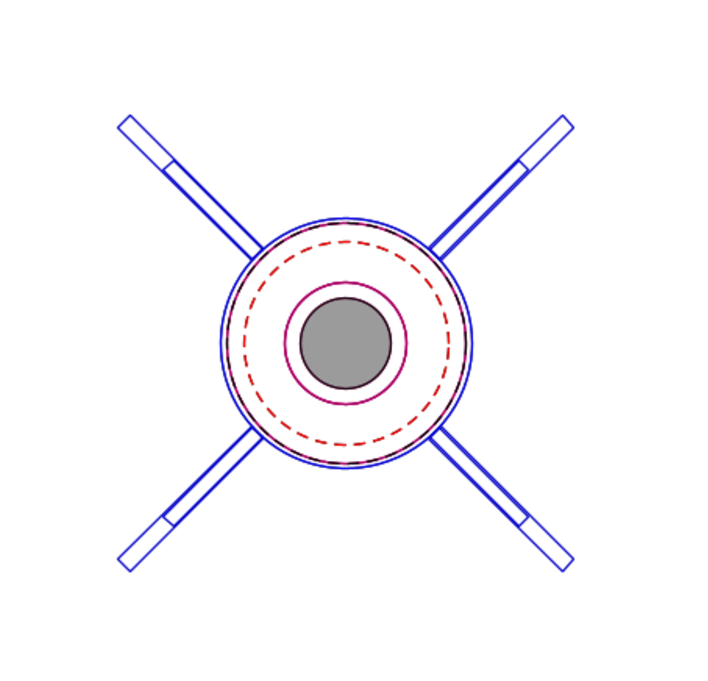
\includegraphics[width=\SchematicWidth]{\Images/mechanical/AileronsPosition.eps}
    \caption{Simulink model we used}
\end{figure}
\FloatBarrier
